\documentclass[english,12pt]{article}
\usepackage[T1]{fontenc}
\usepackage[latin9]{luainputenc}
\usepackage{babel}
\usepackage{array}
\usepackage{float}
\usepackage{amstext}
\usepackage{amssymb}
\usepackage{graphicx}
\usepackage{upgreek}
\usepackage{cite}
\usepackage{titlesec}
\usepackage{pgfgantt}
\usepackage{pgfgantt}
\usepackage{graphicx}
\usepackage{xcolor}
\usepackage{pdfpages}

\setcounter{tocdepth}{4}
\setcounter{secnumdepth}{4}

\titleformat{\paragraph}
{\normalfont\normalsize\bfseries}{\theparagraph}{1em}{}
\titlespacing*{\paragraph}
{0pt}{3.25ex plus 1ex minus .2ex}{1.5ex plus .2ex}


\usepackage[unicode=true,pdfusetitle,
 bookmarks=true,bookmarksnumbered=false,bookmarksopen=false,
 breaklinks=false,pdfborder={0 0 1},backref=false,colorlinks=false] {hyperref}

% copying some latex magic from Yuval
\usepackage{xspace}
\usepackage{color}
\newif\ifNotes\Notestrue
\newcommand{\swallow}[1]{}
\ifNotes
  \newcommand{\colorcomment}[2]{\leavevmode\unskip\space{\color{#1}[#2]}\xspace}
\else
  \newcommand{\colorcomment}[2]{\leavevmode\unskip\relax}
\fi
\newcommand{\taggedcolorcomment}[3]{\colorcomment{#1}{\textbf{#2}: #3}}
\newcommand{\todo}[1]{\colorcomment{red}{TODO: #1}}
\newcommand{\refs}{\colorcomment{red}{REFS}}
\newcommand{\yossi}[1]{\taggedcolorcomment{green}{Yossi}{#1}}
\newcommand{\amit}[1]{\taggedcolorcomment{blue}{Amit}{#1}}



% source: https://tex.stackexchange.com/a/74782
\newcommand\dblquote[1]{\textquotedblleft #1\textquotedblright}
\newcommand\textbfit[1]{\textbf{\textit{#1}}}


\makeatletter

%%%%%%%%%%%%%%%%%%%%%%%%%%%%%% LyX specific LaTeX commands. % Because html
%converters don't know tabularnewline
\providecommand{\tabularnewline}{\\}
%% A simple dot to overcome graphicx limitations
\newcommand{\lyxdot}{.}


%%%%%%%%%%%%%%%%%%%%%%%%%%%%%% User specified LaTeX commands.
\usepackage{graphicx}

\makeatother

\begin{document}
\begin{titlepage}

\newcommand{\HRule}{\rule{\linewidth}{0.5mm}} 
% Defines a new command for the horizontal lines, change thickness here

\center % Center everything on the page
 

%----------------------------------------------------------------------------------------
%	LOGO SECTION
%----------------------------------------------------------------------------------------


\includegraphics[scale=0.025]{images/bgu.png}\\[1cm] 


 
%----------------------------------------------------------------------------------------

%----------------------------------------------------------------------------------------
%	HEADING SECTIONS
%----------------------------------------------------------------------------------------

% Name of your university/college 
\textsc{\LARGE Ben-Gurion University of the Negev}\\[1.5cm] 

\textsc{\Large Faculty of Engineering Science}\\[0.5cm] 

% Major heading such as course name 
\textsc{\large Department of Software and Information Systems
Engineering}\\[0.5cm] 

% Minor heading such as course title 
\textsc{\large Project in Offensive Artificial Intelligence Course}\\[0.5cm] 

% Minor heading such as course title

%----------------------------------------------------------------------------------------
%	TITLE SECTION
%----------------------------------------------------------------------------------------

\HRule \\[0.4cm]
{ \huge \bfseries OAI Final Project - Robustness of Real Time Deepfakes } \\[0.4cm] 
% Title of your document 
\HRule \\[1.5cm]
 
%----------------------------------------------------------------------------------------
%	AUTHOR SECTION
%----------------------------------------------------------------------------------------

\begin{minipage}{0.4\textwidth}
\begin{flushleft} \large \emph{Author:}\\
Amit Kama % Your name
\end{flushleft}
\end{minipage}
~
\begin{minipage}{0.4\textwidth}
\begin{flushright} \large \emph{Author:} \\
Oren Shvartzman % Your Name
\end{flushright}
\end{minipage}\\[3cm]

% \begin{minipage}{0.4\textwidth}
% \begin{flushleft} \large \emph{Author:}\\
% Barak Yacouel % Your name
% \end{flushleft}
% \end{minipage}
% ~
% \begin{minipage}{0.4\textwidth}
% \begin{flushleft} \large \emph{ }\\
%   % Your name
% \end{flushleft}
% \end{minipage}\\[2cm]
    
% If you don't want a supervisor, uncomment the two lines below and remove the
% section above \Large \emph{Author:}\\
% John \textsc{Smith}\\[3cm] % Your name

%----------------------------------------------------------------------------------------
%	DATE SECTION
%----------------------------------------------------------------------------------------

{\large \today}\\[3cm] 
% Date, change the \today to a set date if you want to be precise


\vfill % Fill the rest of the page with whitespace

\end{titlepage}

\pagebreak{}


\tableofcontents{}

\pagebreak{}


\section{Introduction} \label{introduction}

% Deepfakes and deepfakes in recent years
Deepfake is a general term that encompasses the use of deep learning algorithms in order to create
synthetic media, in which one subject in an existing visual and/or audio content is usually replaced
with another's likeness. While fraudulent content has been around for some time, recent advances in
machine vision have posed a major threat to the trust and transparency of the media. Using powerful
machine-learning and deep-learning techniques, deepfakes can now manipulate or generate visual and
audio content that can be more easily misleading.

In recent years, deepfakes have garnered widespread attention for their uses in spreading fake news,
committing financial fraud, creating pornographic materials, and many other disturbing uses. This has
led to a significant need to identify and restrict their use.

% First Order Model
Ever since the introduction of deepfakes, researchers in deep learning have increasingly focused on
this area of research. In particular, they propose methods, as well as practical implementations of
deepfakes is in various fields. Among other methods, in~\cite{DBLP:journals/corr/abs-2003-00196}, Siarohin et al. propose
the first order motion model for image animation. Their framework enables generating a video sequence,
in which an object in a source image is animated according to the motion of a driving video, without
using any annotation or prior information about the specific object to animate. According to them,
once trained on a set of videos depicting objects of the same category, the method can be applied
to any object of it. Based on this method, a number of real time photorealistic avatars have recently
been developed, one of which we will explore in this work.

% It has limitations - drawbacks, that in the literature, there is a growing amount of research dealing with the field.
However, real time avatars are far from perfect, as they are not robust when it comes to edge cases.
This includes facial gestures in the driving video, objects in the source or target media that make it
difficult to identify facial boundaries, and many more.


% Detection (Importance, ways)
Note that these limitations can create visual glitches and distortions that can be detected with the
naked eye as well as by software, and therefore can be utilized for failures detection. This observation
drives a growing amount of research dealing with those inaccuracies for dual use -- correcting them in
order to improve the deepfakes' credibility, or exploiting them to distinguish deepfakes from real content.

% What will be in the report
In this work, we evaluate the robustness of real time deepfakes by implementing first order motion
model-based avatarify and examining various edge cases on it. After demonstrating failures in the
implementation, we also provide a method to utilize them for failures detection.


% \pagebreak{}

\section{Methods} \label{methods}

In this section we will briefly introduce the First Order Motion Model, on which the avatarify implementation
whose robustness we evaluated, consists of. In addition, we will describe our proposed method for failures detection.

% Detailed explanation on First Order Model
\subsection{First Order Motion Model} \label{implementation}
% From DBLP:journals/corr/abs-2003-00196
% The method, our plan to evaluate it
%+++++++++++++++++++++++++++++++++++++++++++++++++++++++++++++++++++++++++++++++++++++++++++++++++++++++++++++++++++++++

% FIXME: Do we want to add figures from the paper?

In~\cite{DBLP:journals/corr/abs-2003-00196}, Siarohin et al. propose the First Order Motion Model for Image
Animation, which addresses the task of generating a video sequence so that an object in a source image
is animated according to the motion of a driving video.

Once their proposed method is trained on a set of videos depicting objects in the same category, it can be
applied to any object in this category, without using annotations or prior knowledge about the object to be
animate.
This is done using a self-supervised formulation, for detaching appearance information and motion information
from each other. The method also supports complex motions, using representation consisting of a set of learned
keypoints along with their local affine transformations.

The model's mathematical formulation describes motion between two frames and is efficiently computed by
deriving a first order Taylor expansion approximation. Thus, motion is represented as a set of keypoints
displacements and local affine transformations.
Finally, a generator network combines the appearance extracted from the source image with the motion
representation of the driving video. First Order Motion Model outperforms state of the art on all the
benchmarks on a variety of object categories.

In the background of this method, most of the works that appear in the literature tackle image animation
task by assuming strong priors on the object representation and resorting to computer graphics techniques.
Such methods can be described as object-specific methods, due to the knowledge that they assume on the
model of the specific object to animate.

Recent works of deep generative models have derived various techniques for image animation, such as
Generative Adversarial Networks (GANs) and Variational Auto-Encoders (VAEs) for facial expressions
transfer or motion patterns between human subjects in videos. Having said that, these methods
usually also use pre-trained models to extract object-specific representations.

However, these models consist of costly ground truth data annotations, and are not available in general
for an arbitrary object category. Siarohin et al. address these issues with more object-agnostic approach.
As they use a set of self-learned keypoints with local affine transformations to model complex motions,
they call the method the First Order Motion Model.\\

% \begin{figure}[htb]
%   \begin{centering}
%       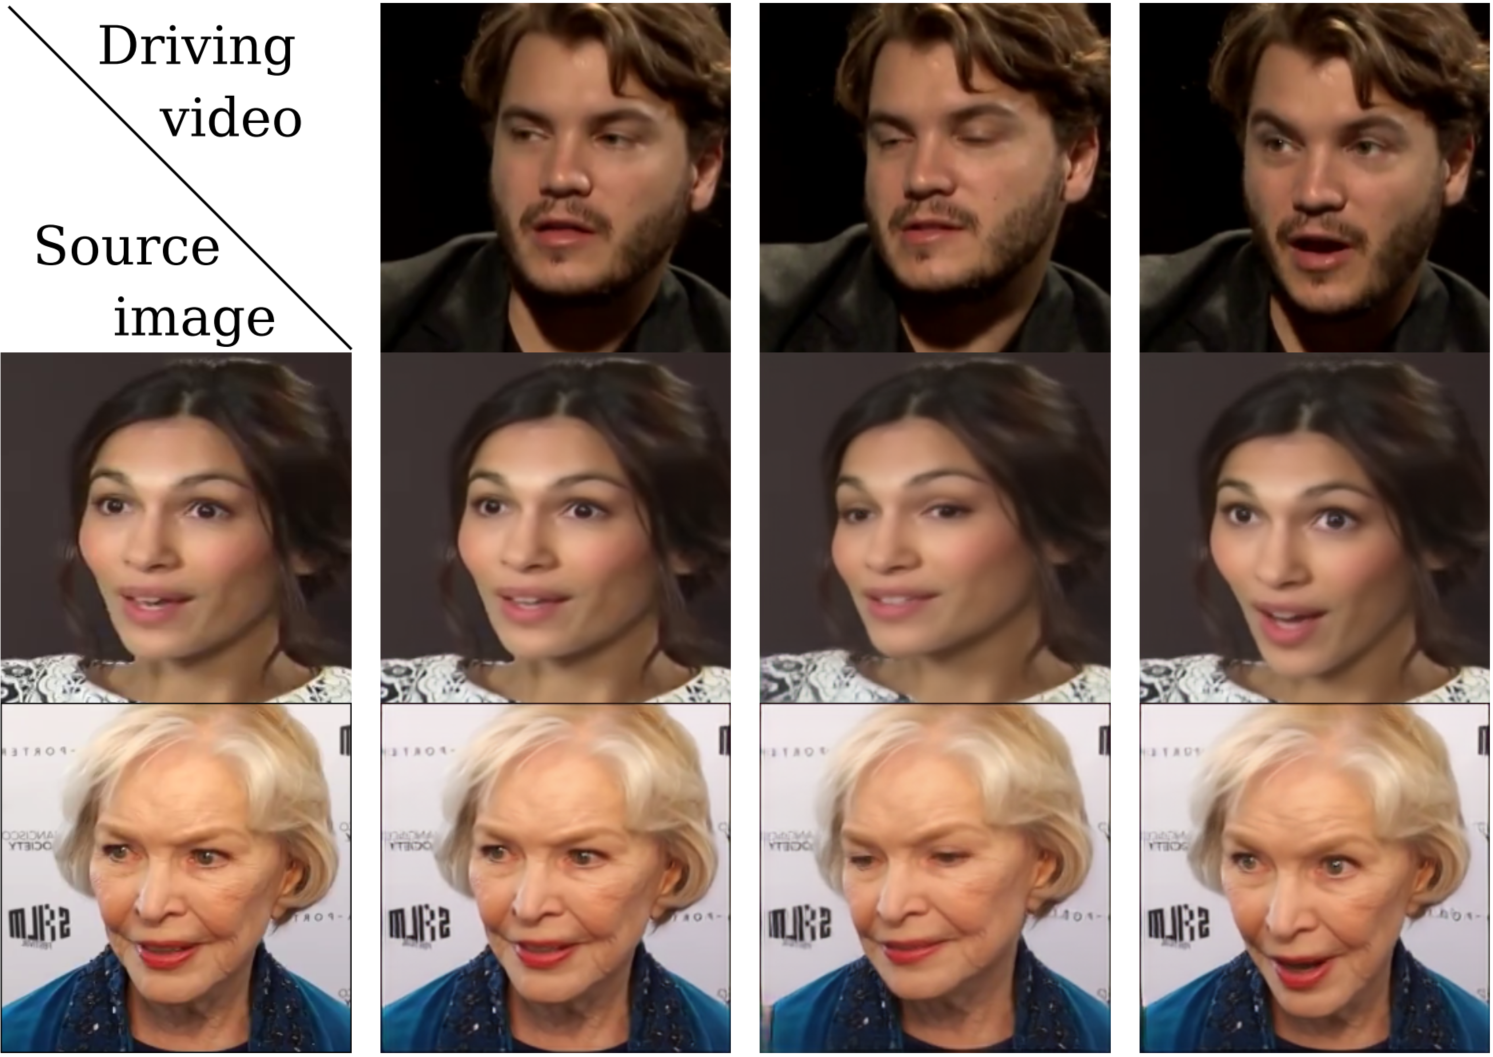
\includegraphics[scale=0.2]{images/‏‏example.PNG}
%   \par\end{centering}
%   \caption{\label{fig:first_figure}Example animations produced by the First Order Motion Model trained on VoxCeleb dataset [22] using relative motion transfer.~\cite{DBLP:journals/corr/abs-2003-00196}}
% \end{figure} 

\begin{figure}[htb]
  \begin{centering}
      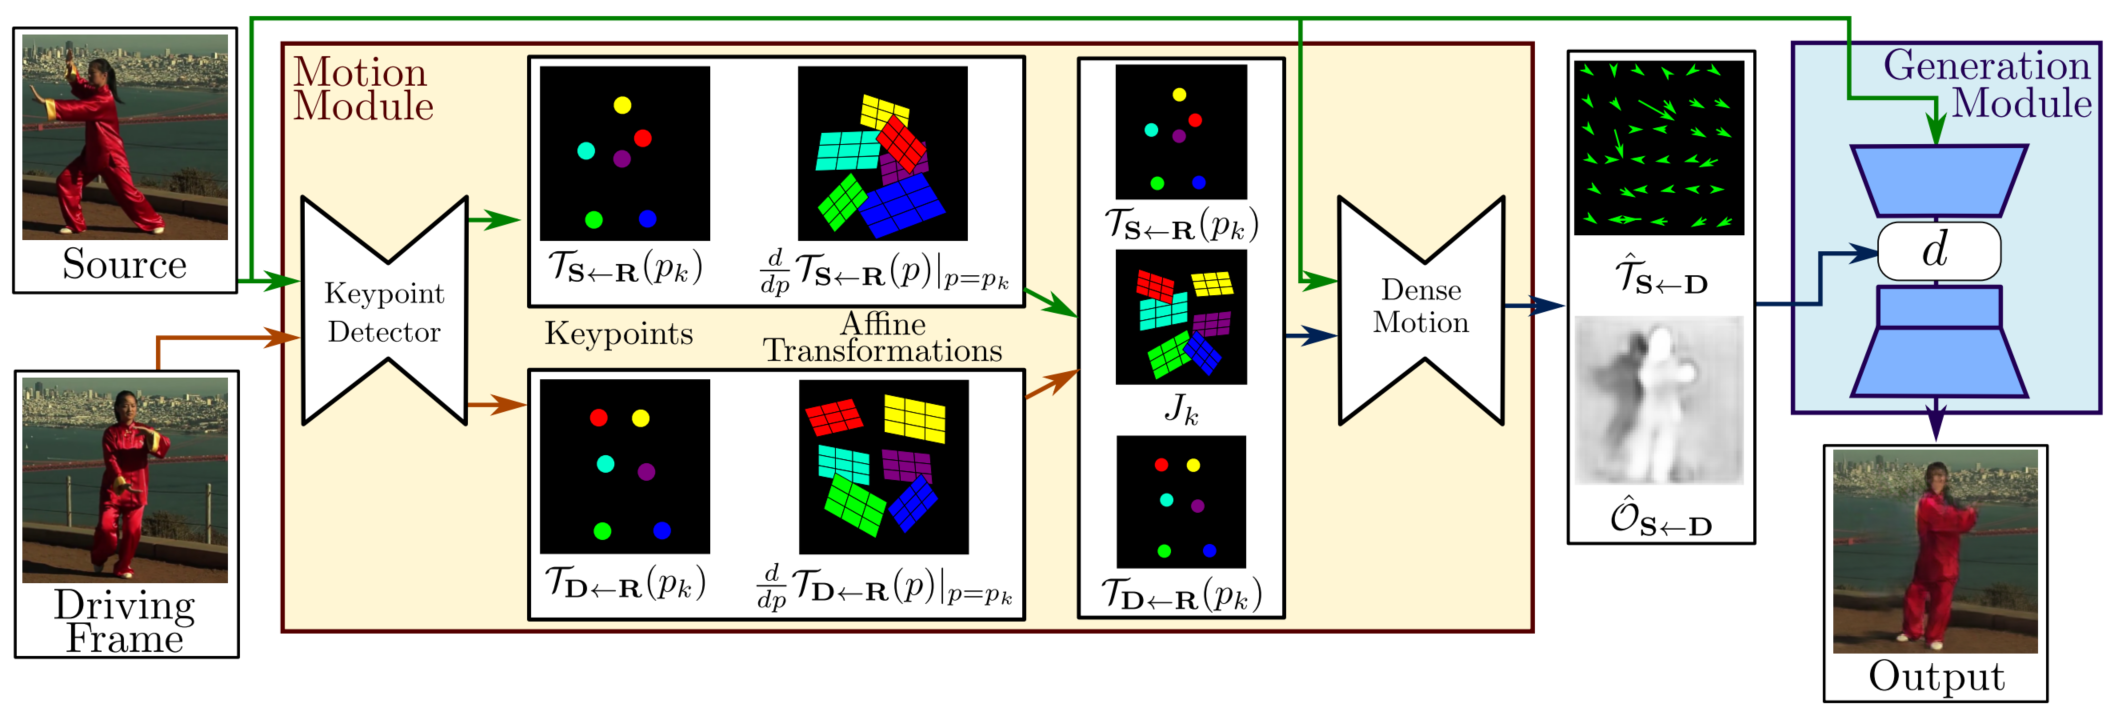
\includegraphics[scale=0.24]{images/method.PNG}
  \par\end{centering}
  \caption{\label{fig:second_figure}Overview of the First Order Motion Model approach. The model gets as inputs a source image S and a frame of a driving video frame D. Using unsupervised keypoint detector the motion model extracts first order motion
  representation consisting of keypoints displacements and local affine transformations with respect to a reference frame R. Using the motion representation a dense
  motion network generates dense optical flow \^T from D to S and occlusion map \^O from D to S. Lastly, using the source image and the dense motion network's outputs, a generator renders the target image.~\cite{DBLP:journals/corr/abs-2003-00196}}
\end{figure} 




%+++++++++++++++++++++++++++++++++++++++++++++++++++++++++++++++++++++++++++++++++++++++++++++++++++++++++++++++++++++++

% Explanation on our proposed method
\subsection{Failures Detection Method}
% \subsubsection{Facial Detection with Dlib}
At the basis of our method for failures detection is the idea according to which we can detect
the avatarify failures using anomaly detection methods. To address the task of detecting avatarify
failures in an output video, we simplified it to the problem of detecting avatarify failures in a
target image. To do so, the method starts with dividing the video into several frames.
For each frame we extract the facial landmarks, calculate Euclidean distance between all the points.
We then normalize and run the results through the local outlier factor model with 20 neighbors.
Note that we extract the facial landmarks using Dlib~\cite{Dlib, github}, a modern toolkit which contains machine learning
algorithms and tools for creating complex software to solve real world problems. Among many major features
that Dlib provides, there is a high quality face recognition capability.
The test is done using the Yale Face Database~\cite{Yale}, which contains 165 grayscale images in GIF format of
15 individuals, when for each subject, there are 11 images, one for each different facial expression or
configuration: center-light, w/glasses, happy, left-light, w/no glasses, normal, right-light, sad, sleepy,
surprised, and wink. This is in practice using novelty local outlier factor, since the dataset contains only ordinary faces.

The test includes making prediction on each frame of the video. If one or more frames are considered anomalies,
we declare the video to be deepfake.\\

\begin{figure}[htb]
  \begin{centering}
      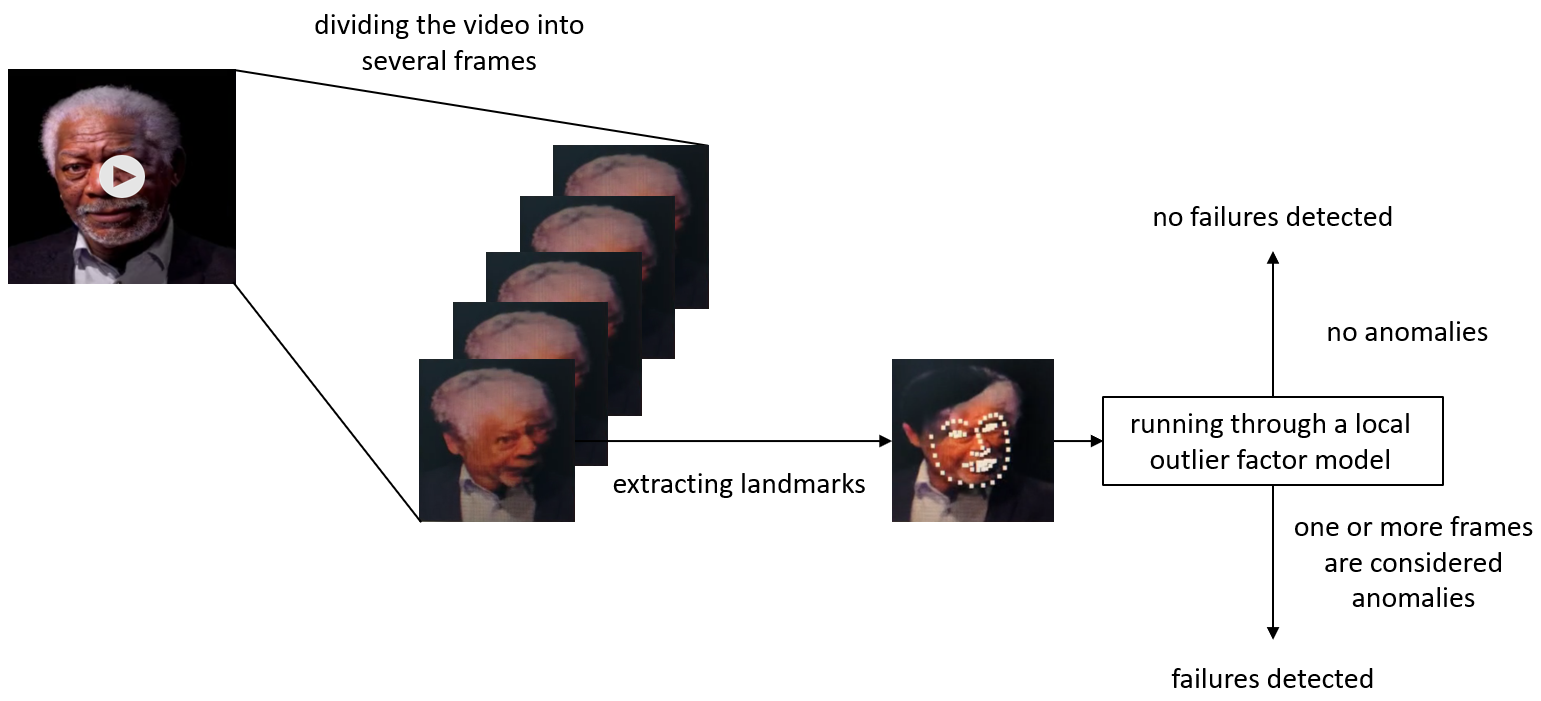
\includegraphics[scale=0.34]{images/our.PNG}
  \par\end{centering}
  \caption{\label{fig:method}Overview of our proposed failures detection method.}
\end{figure}


\section{Experiments and Results} \label{experiments and results}

In this section we introduce the experiments and results. A detailed explanation of the
visual glitches and distortions that we managed to create and detect is provided, as well
as the results of our proposed method to utilize them for failures detection.

% examples for edge cases on the Avatarify
\subsection{First Order Model Robustness}

In order to evaluate the robustness of real time deepfakes, we started by implementing
avatarify and then examining edge cases on it. We implemented the First Order Motion Model
mentioned in \ref{implementation}.

Since we focused on the implementation of avatarify which work in a way that a face in a source
image is animated according to the motion of a driving video, we tried to test its limitations
by passing driving videos with various facial gestures and head tilt as input. This includes
winks, tongue out, smiles, eyebrow raise, different head tilts, etc.

From the output videos, it was clear that the avatarify does not work on certain artifacts.
For example, avatarify is not able to create videos with a tongue out at all, as well as
creating a proper dental structure. However, even when it fails to copy certain facial gestures
to a source image perfectly, the outputs still look relatively believable.

The more significant limitation we identified in the implementation, is the creation of a video
that includes head tilts, or more precisely, that the extraction of the keypoints from the faces
in the input videos is more complex.\\


\begin{figure}[htb]
  \begin{centering}
      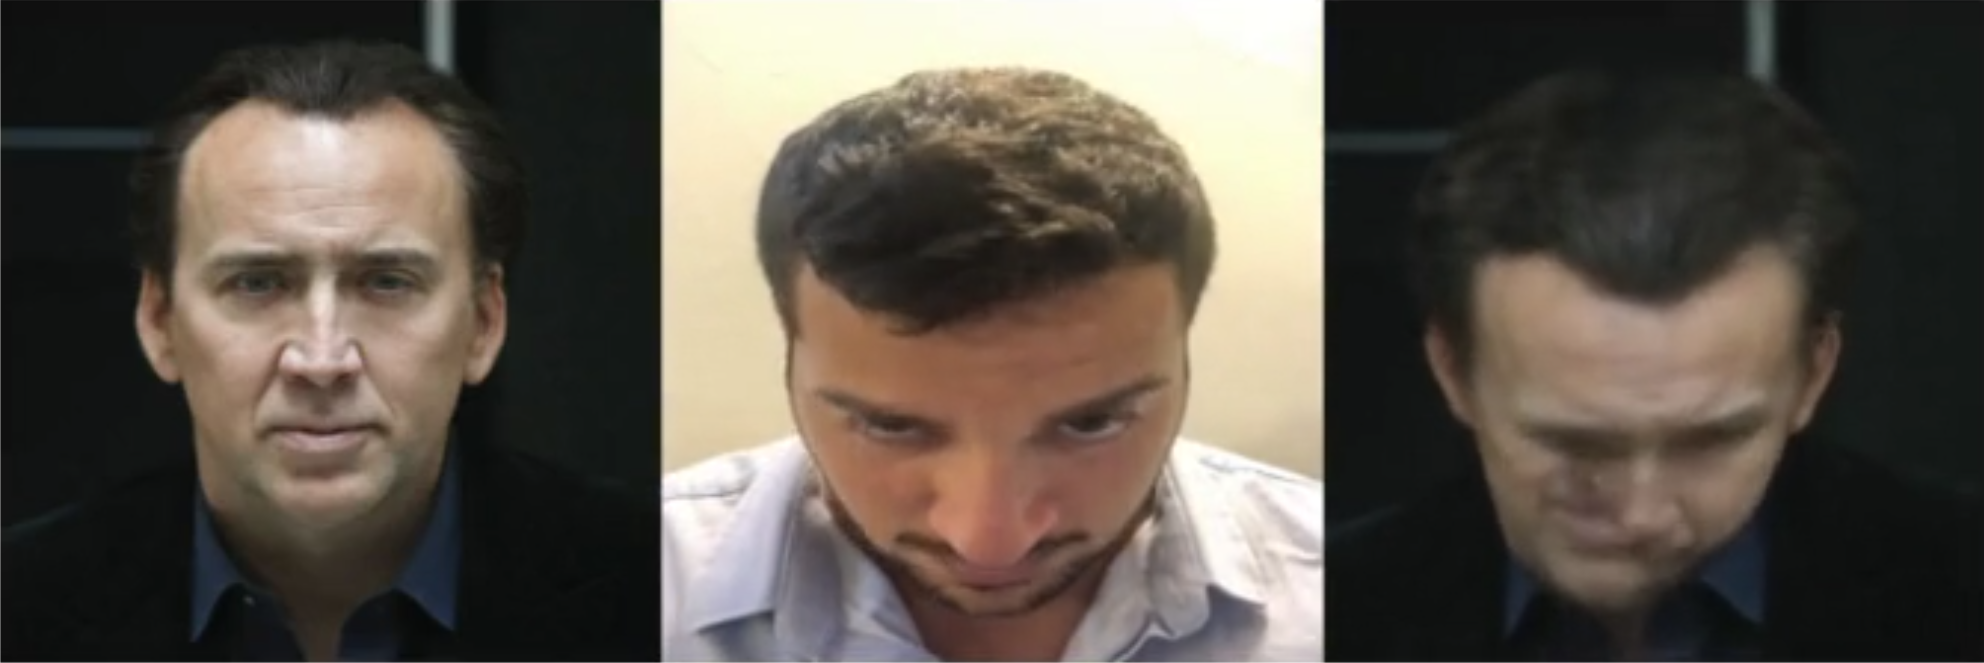
\includegraphics[scale=0.25]{images/‏‏Amit_tilt1_cage.PNG}
  \par\end{centering}
  \caption{\label{fig:Amit_tilt1_cage}The output consists of a source image of Nicolas Cage and a driving video which includes head tilt. It can be seen that the avatarify failed to generate a reliable output.}
\end{figure}

% \begin{figure}[htb]
%   \begin{centering}
%       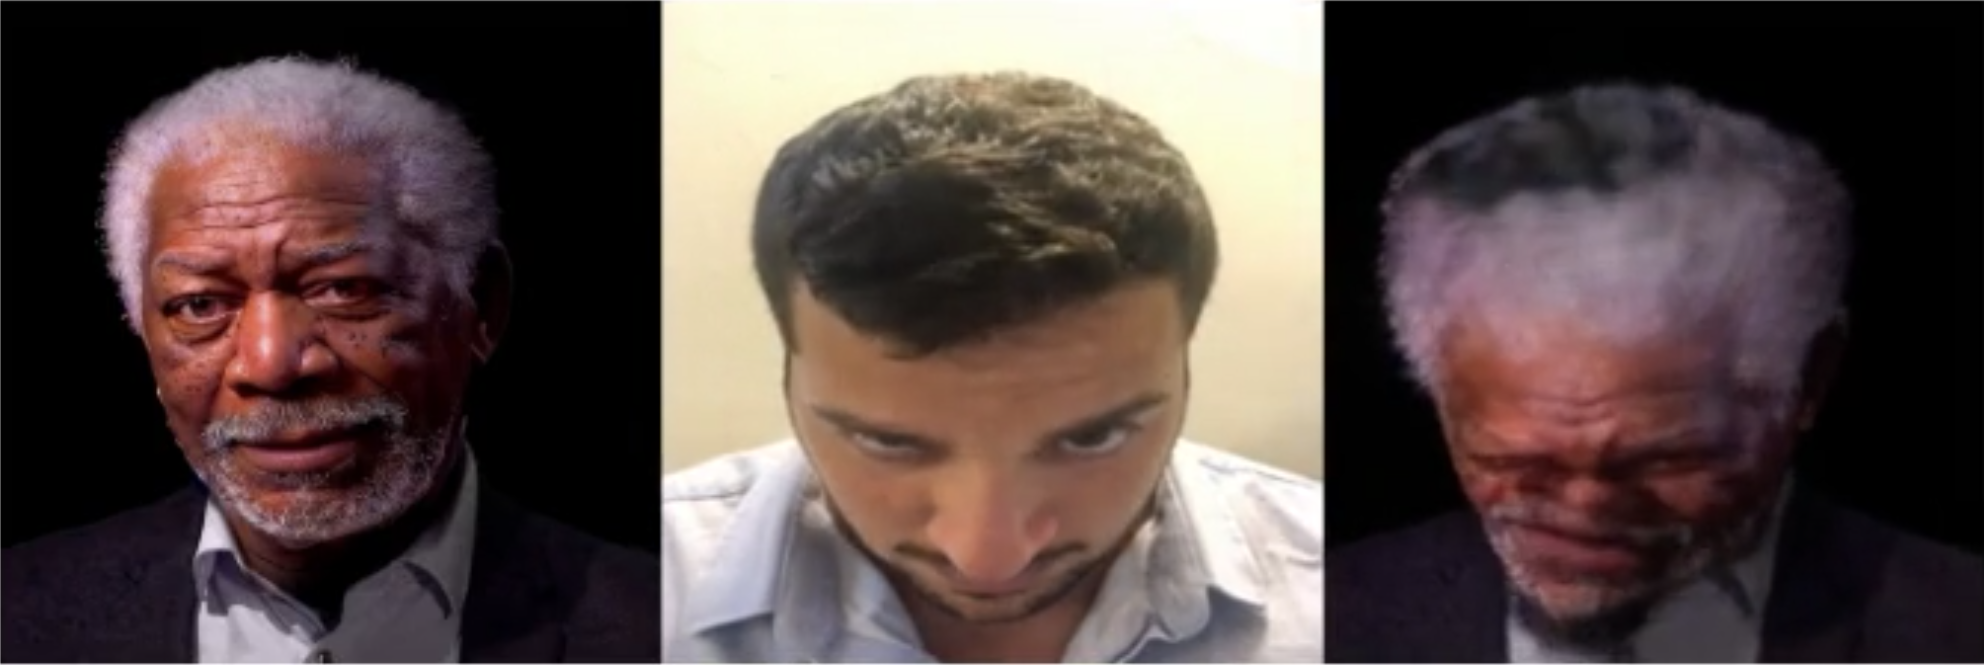
\includegraphics[scale=0.25]{images/‏‏Amit_tilt1_freeman.PNG}
%   \par\end{centering}
%   \caption{\label{fig:Amit_tilt1_freeman}The effect of...}
% \end{figure}

% \begin{figure}[htb]
%   \begin{centering}
%       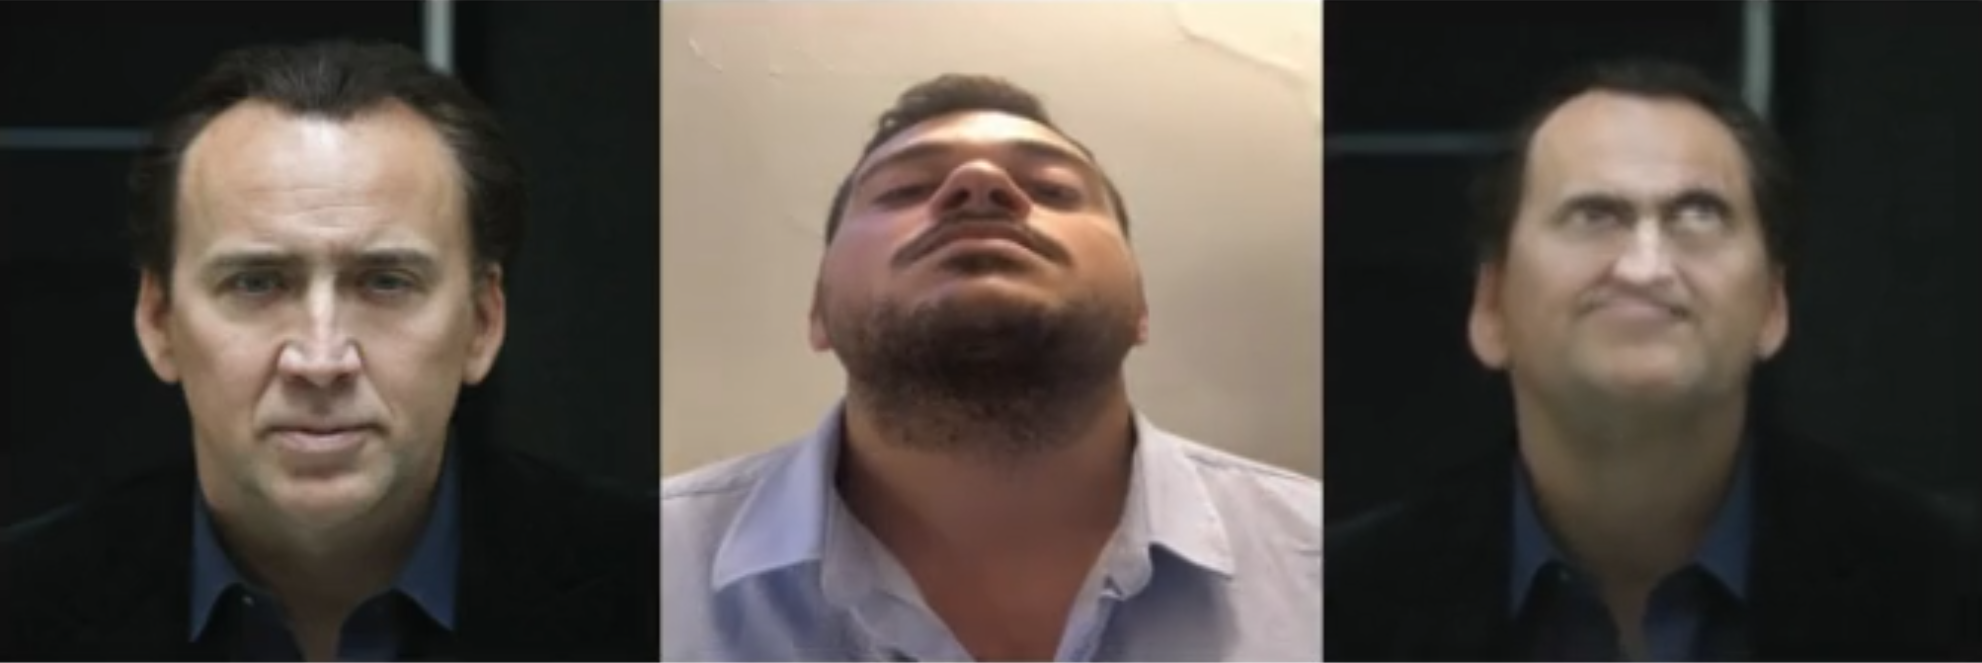
\includegraphics[scale=0.25]{images/‏‏Amit_tilt_cage.PNG}
%   \par\end{centering}
%   \caption{\label{fig:Amit_tilt_cage}The effect of...}
% \end{figure}

\begin{figure}[htb]
  \begin{centering}
      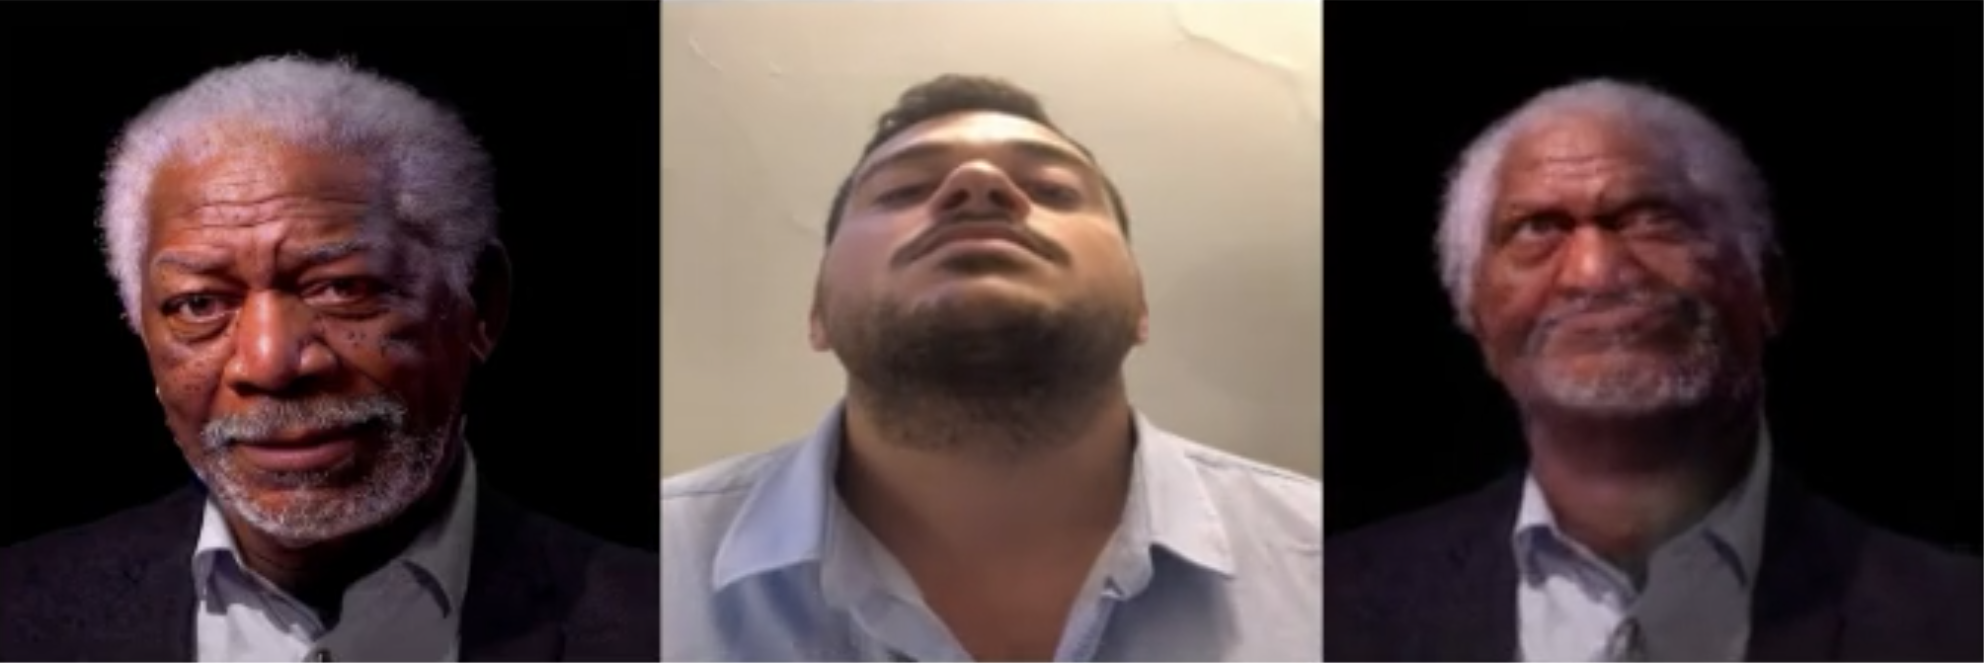
\includegraphics[scale=0.25]{images/‏‏Amit_tilt_freeman.PNG}
  \par\end{centering}
  \caption{\label{fig:Amit_tilt_freeman}The output consists of a source image of Morgan Freeman and a driving video which includes head tilt. It can be seen that the avatarify failed to generate a reliable output.}
\end{figure}

\begin{figure}[!htb]
  \begin{centering}
      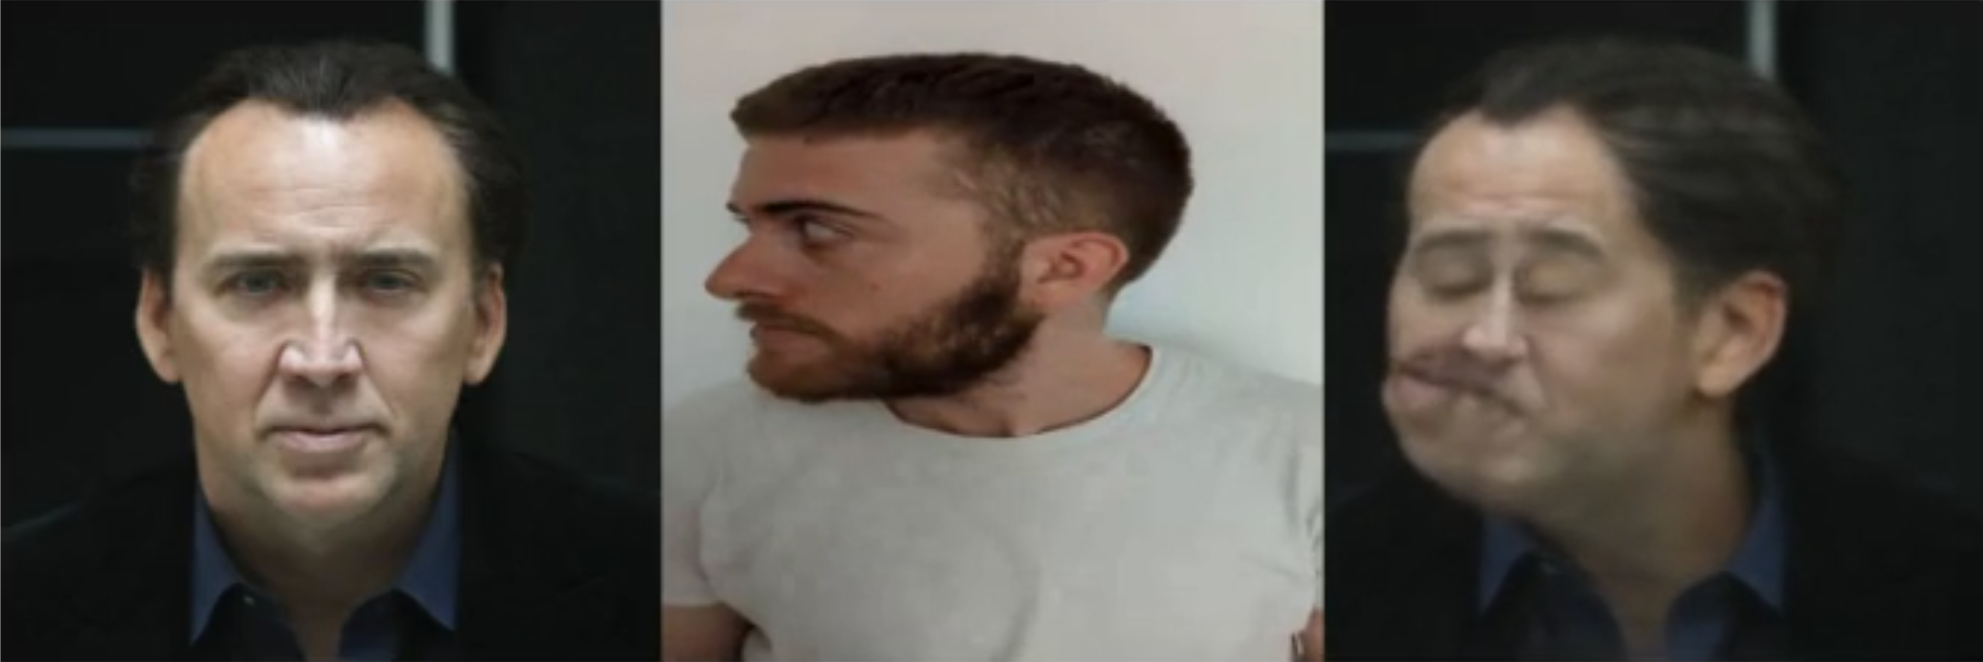
\includegraphics[scale=0.25]{images/Oren_tilt_cage.PNG}
  \par\end{centering}
  \caption{\label{fig:Oren_tilt_cage}The output consists of a source image of Nicolas Cage and a driving video which includes head tilt. It can be seen that the avatarify failed to generate a reliable output.}
\end{figure}
% \pagebreak{}

% \begin{figure}[htb]
%   \begin{centering}
%       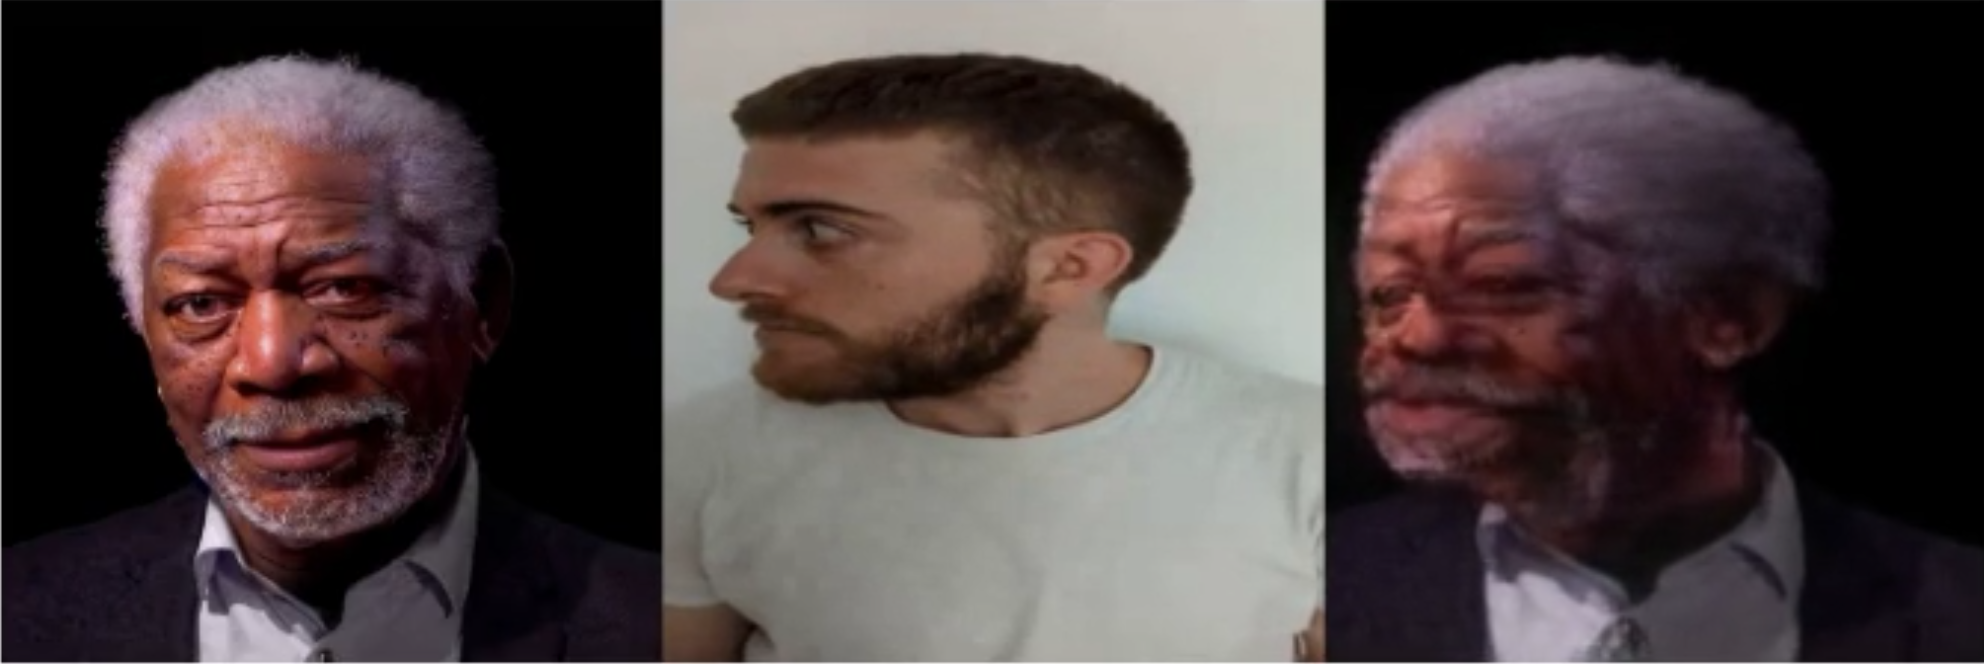
\includegraphics[scale=0.25]{images/Oren_tilt_freeman.PNG}
%   \par\end{centering}
%   \caption{\label{fig:Oren_tilt_freeman}The effect of...}
% \end{figure}

The implementation, including the experiments and results can be found using the following link:\\
https://colab.research.google.com/drive/1oI4jPx9cB26OsCerUs2JfxyGkffBWM5v


\pagebreak{}

\subsection{Failures Detection}

In order to test our proposed method, we fed it with two videos -- authentic video and a deepfake of Morgan Freeman,
derived from the authentic video as a driving video using the First Order Motion model. When we ran the method on
each of the two videos, we found that indeed no failures were detected in the original video, while in the deepfake they were.

\begin{figure}[!htb]
  \begin{centering}
      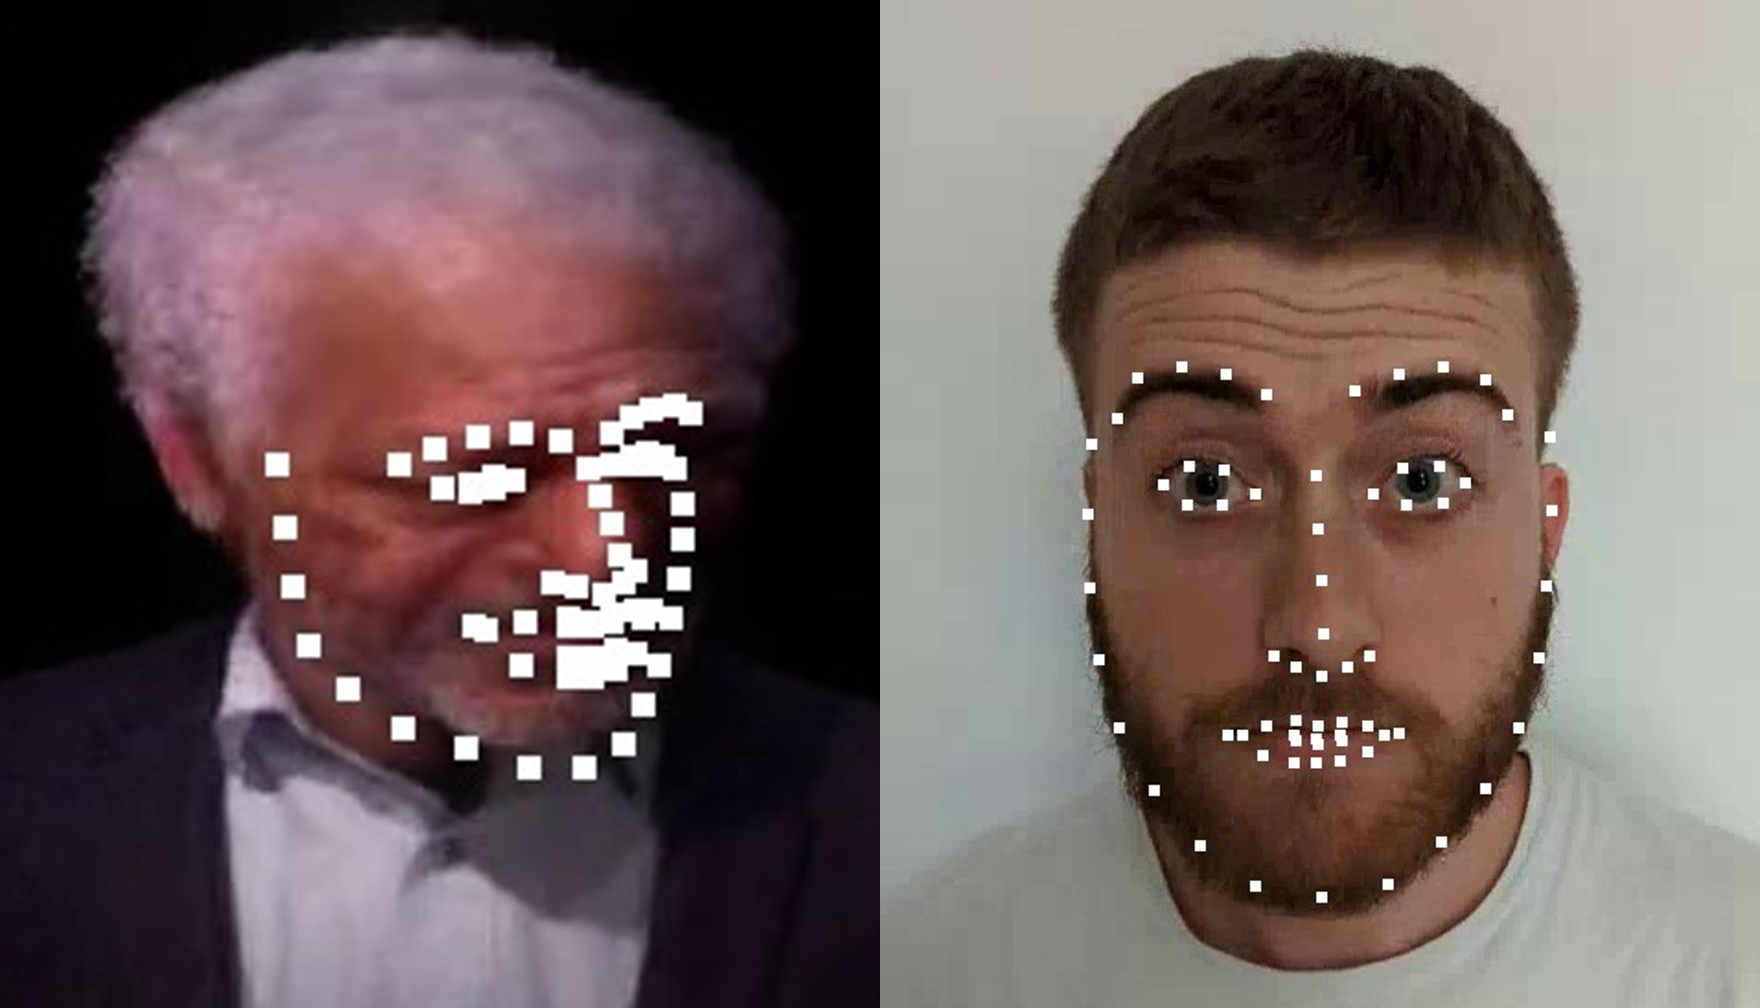
\includegraphics[scale=0.6]{images/oren.png}
  \par\end{centering}
  \caption{\label{fig:Oren}An example of the facial landmarks extraction. Using the local outlier factor model, the left image's landmarks considered anomalies, while in the right image no failures was found.}
\end{figure}

Note that in some cases the face in the target image is distorted enough that it is not possible to identify the face,
and therefore to determine the landmarks. This fact can be exploited for further improvements in the failure detection task.


% \pagebreak{}

\section{Discussion} \label{discussion}

As the impact of social media on our world grows moment by moment, along with the negligible cost
and lack of need for experience enabling almost anyone to create high quality deepfakes, this
emerging technology poses a serious threat to society.

For this reason, in academia and industry there is an extensive practice in this technology, and
they offer many developments, both for improving the quality of deepfake applications and conversely,
mechanisms for dealing with this phenomenon.

In this work we experimented with an implementation of real time deepfakes, the first order motion
model-based avatarify, proposed by Siarohin et al.~\cite{DBLP:journals/corr/abs-2003-00196}, and
evaluated its robustness by examining various end cases on it.

We have learned that avatarify implementations are not robust, and that various facial gestures
and artifacts can cause significant failures in the target videos. It seems that most failures
caused by head tilt and rotations in the driving video, as well as gestures which include objects
that the model does not recognize in the source image, such as tongue or teeth.

After demonstrating failures in the implementation, we also provided a method to utilize them for
failures detection. We were able to successfully demonstrate our method on two videos -- authentic
video and a deepfake. No failures were detected in the original video, while in the
deepfake they were.


\pagebreak{}
\pagebreak{}

\bibliographystyle{plain}
\bibliography{Proposal}

\end{document}